\documentclass{article}
\usepackage[UTF8]{ctex}
\usepackage{amsmath,mathtools,geometry,tikz,enumitem,caption}
\geometry{a4paper,scale=0.7}

\title{每日一题(12.2)}
\author{\kaishu 程昊一、王一丁}

\begin{document}
\maketitle
\textbf{1. }已知:
\begin{enumerate}[noitemsep,label=(\arabic*) ]
	\item\textbf{\kaishu 平行公设: }{\fangsong 同平面内一条直线和另外两条直线相交, 若在直线同侧的两个内角之和小于$180^\circ$, 则这两条直线经过无限延长后在这一侧相交.}\\
	\rightline{\kaishu ———《几何原本》}
	\item\textbf{\kaishu 内角和定理: }{\fangsong 任意一个三角形的内角和为$180^\circ$.}
\end{enumerate}
求证: 平行公设与内角和定理是\textbf{等价的}.\\
\rightline{\kaishu(程昊一供题)}\\\par
\textbf{2. }如图, 在$\Delta ABC$中, $\angle ABC$与$\Delta ABC$的平分线相交于$I$. 过点$I$作$EF\parallel BC$分别交$AB$、$AC$于$E$、$F$. 若$\angle BIC=130^\circ$, $\angle ABC:\angle ACB=3:2$, 求$\angle AEF$和$\angle EFC$.
\rightline{\kaishu (王一丁供题)}
\begin{figure}[htbp]
	\centering
	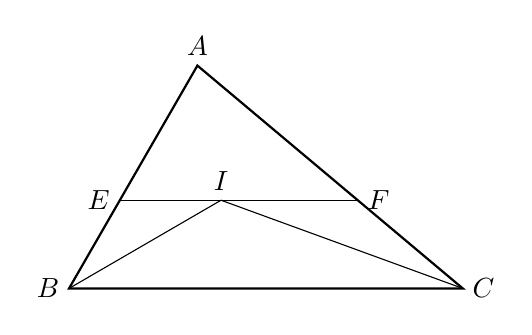
\begin{tikzpicture}
		\draw [thick](0,0)--(5,0)--(1.63,2.83)--cycle;
		\draw (0,0)--(1.93,1.12);
		\draw (5,0)--(1.93,1.12);
		\draw (0.64,1.12)--(3.67,1.12);
		
		\node at (0,0) [left] {$B$};
		\node at (5,0) [right] {$C$};
		\node at (1.63,2.83) [above] {$A$};
		\node at (1.93,1.12) [above] {$I$};
		\node at (0.64,1.12) [left] {$E$};
		\node at (3.67,1.12) [right] {$F$};
	\end{tikzpicture}
	\caption*{\kaishu 第二题图}
\end{figure}
\end{document}